\documentclass[11pt, letterpaper]{article}
\usepackage[utf8]{inputenc}
\usepackage[margin=1in]{geometry}
\usepackage{enumitem}
\usepackage{indentfirst}
\usepackage{titling}
\usepackage{graphicx}
\usepackage{amsmath}
\usepackage{amsfonts}
\usepackage{amsthm}
\usepackage{mathtools}
\usepackage{hyperref}
\usepackage{mathabx}
\usepackage{caption}
%\usepackage{subcaption}
\usepackage{bm}
\usepackage{textcomp}
\usepackage{subfig}
\usepackage[dvipsnames]{xcolor}
\graphicspath{ {./} }
\DeclareMathAlphabet{\altmathcal}{OMS}{cmsy}{m}{n}

\newtheorem{theorem}{Theorem}[subsection]
\newtheorem{corollary}{Corollary}[theorem]
\newtheorem{lemma}[theorem]{Lemma}

\theoremstyle{definition}
\newtheorem{definition}{Definition}[subsection]

\theoremstyle{remark}
\newtheorem*{remark}{Remark}

\newcommand{\bv}[2][]{\bm{\vec{#2}_{#1}}}

\setlength{\parindent}{0cm}
\setlength{\parskip}{1em}
\renewcommand{\baselinestretch}{1.5}

\hypersetup{
    colorlinks=true,
    linkcolor=cyan,
    filecolor=magenta,      
    urlcolor=blue,
}

\title{Chapter VIII: Introduction to Magnetism}
\author{Chenyi Zhu}
\date{March 27th, 2020}

\begin{document}


\begin{titlingpage}
	\maketitle
	
	\begin{figure}[h!]
		\centering
		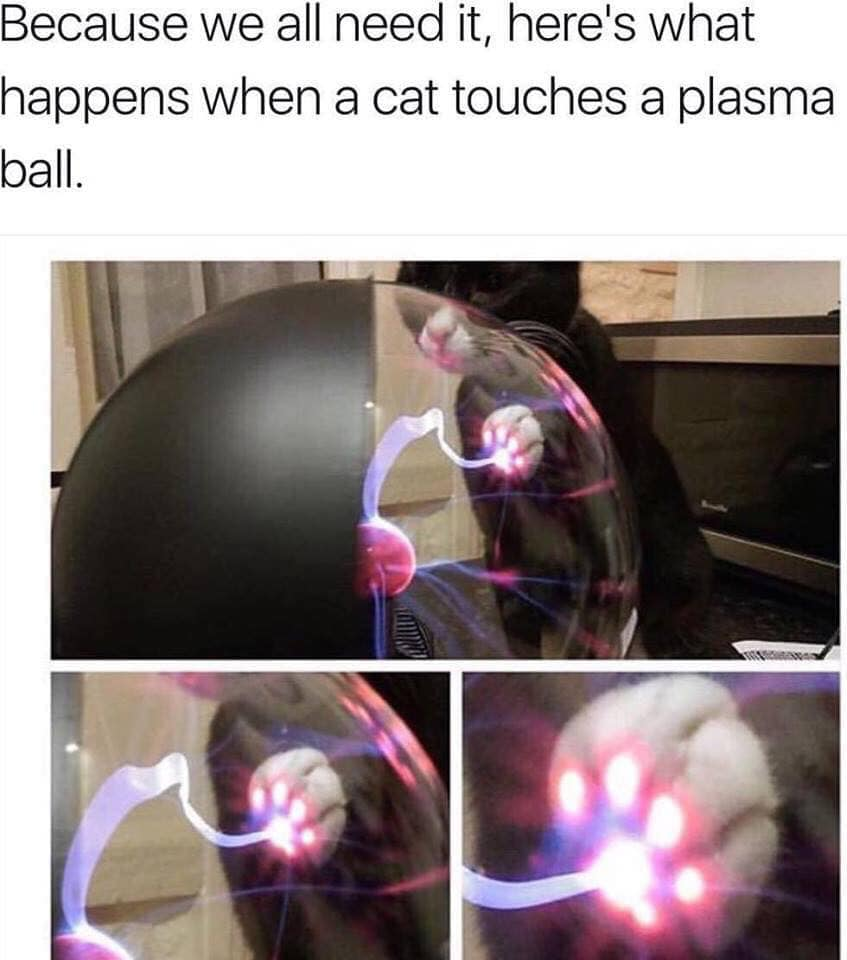
\includegraphics[scale=0.3]{cat}
		\label{fig:flux}
	\end{figure}
		
\end{titlingpage}

\section{Introduction.}
We have seen that a charged object produces an electric field $\bv{E}$ at all points in space. Similarly, a magnet is a source of a magnetic field $\bv{B}$, which you can show by moving it close to a magnet. Magnets consist of two poles, the north and the south. However, unlike electric charges which can be isolated, magnetic poles always come in a pair. Breaking the bar magnet results in two new bar magnets, each with a north and south pole. Magnetic monopoles do not exist in isolation, but are of theoretical interests. We cannot define magnetic field $\bv{B}$ the same way as the electric field $bv{E}$ \[\bv{E} = \frac{\bv[e]{F}}{q}\] due to the lack of magnetic monopoles. 

\section{Definition of Magnetic Fields.}
To define the magnetic field at a point, consider a particle of charge $q$ and moving at a velocity $\bv{v}$. From experimental data we have the following observations:
\begin{itemize}
	\item The magnitude of the magnetic force $\bv[B]{F}$ exerted on the charged particle is proportional to both $\bv{v}$ and $q$;
	\item The magnitude and direction of $\bv[B]{F}$ depends on $\bv{v}$ and $\bv{B}$;
	\item The magnetic force $\bv[B]{F}$ vanishes when $\bv{v}$ is parallel to $\bv{B}$. However, when $\bv{v}$ makes an angle $\theta$ with $\bv{B}$, the direction of $\bv[B]{F}$ is perpendicular to the plane formed by $\bv{v}$ and $\bv{B}$, and the magnitude of $\bv[B]{F}$ is proportional to $\sin{\theta}$;
	\item When the sign of the charge of the particle is switched from positive to negative (or vice versa), the direction of the magnetic force also reverses.
\end{itemize}
All of the above can summarize to one simple expression: 
\begin{equation}\label{eqn:magnetic-force}
	\boxed{\bv[B]{F} = q\bv{v}\times\bv{B}}
\end{equation}
This expression is a working definition of the magnetic field at a point in space. The magnitude $|\bv[B]{F}|$ is then: \[F_B = |q|vB\sin{\theta}\] and the SI unit of magnetic field is the tesla ($T$): \[1\, T = 1\,\frac{N}{C\cdot m/s} = 1\,\frac{N}{A\cdot m}\] Another commonly used non-SI unit for $\bv{B}$ is the gauss ($G$), where $1\, T = 10^4\,G$. 

By convention, for magnetic field lines pointing 

\textbf{Note}: $\bv[B]{F}$ is always perpendicular to $\bv{v}$ and $\bv{B}$, and cannot change the particle's speed $v$ (and thus kinetic energy as well), i.e. magnetic forces cannot speed up or slow down a charged particle. Consequently, $\bv[B]{F}$ can do no work on the particle: \[dW = \bv[B]{F}\cdot\, d\bv{s} = q(\bv{v}\times\bv{B})\cdot\bv{v}\, dt = q(\bv{v}\times\bv{v})\cdot\bv{B}\, dt = 0\] The direction of $\bv{v}$, however, can be altered y the magnetic force, and we shall show that now.

\section{Magnetic Force on a Current-Carrying Wire.}
We have just seen that a charged particle moving through a magnetic field experiences a magnetic force $\bv[B]{F}$. Since electric current consists of a collection of charged particles \textbf{in motion}, when placed in a magnetic field, a current-carrying wire will also experience a magnetic force. Let's look at an example. 

Consider a long straight wire suspended in the region between the two magnetic poles. The magnetic field points out of the page and is represented with dots ($\bullet$, otherwise $\times$). When a downward current passes through, the wire is deflected to the left. However, if we send a current upwards, the wire will be deflected to the right.
\begin{figure}[h!]
		\centering
		\subfloat{{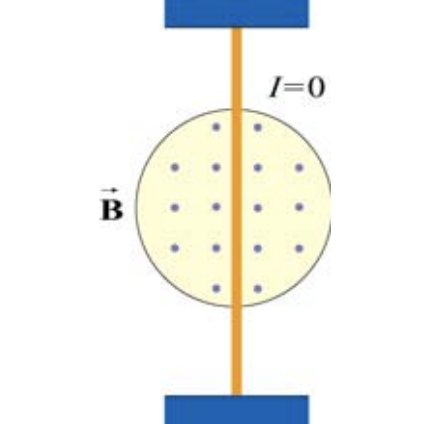
\includegraphics[width=3cm]{middle.png}}}
		\qquad
		\subfloat{{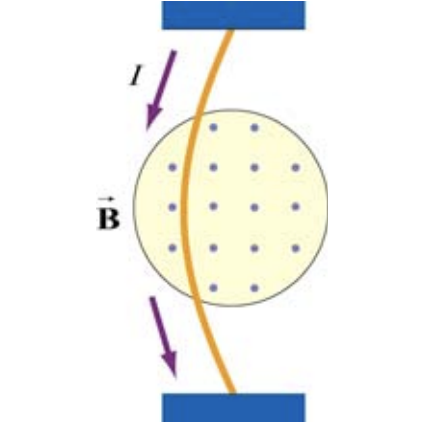
\includegraphics[width=3cm]{left.png}}}
		\qquad
		\subfloat{{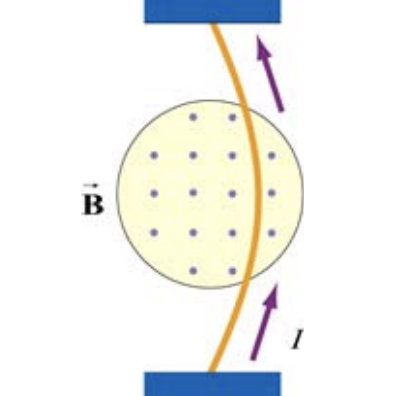
\includegraphics[width=3cm]{right.png}}}
		\caption{Current-carrying wire in a magnetic field.}
\end{figure}

To calculate the force exerted on the wire, consider a segment of wire of length $l$ and cross-sectional area $A$. The magnetic field points into the page. 
\begin{figure}[h!]
	\centering
	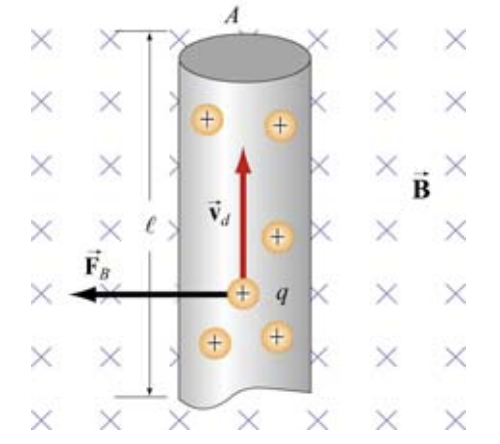
\includegraphics[scale=0.6]{wire}
	\caption{Magnetic force on a conducting wire.}
	\label{fig:wire}
\end{figure}

The charges move at an average drift velocity $\bv[d]{v}$. Since the total amount of charge in this segment is $Q_{tot} = q(nAl)$, where $n$ is the number of charges per unit volume (recall from chapter $5$ section on current density), the total magnetic force on the segment is \[\bv[B]{F} = Q_{tot}\bv[d]{v}\times\bv{B} = qnAl(\bv[d]{v}\times\bv{B}) = I(\bv{l}\times\bv{B})\] where $I = nqv_dA$, and $\bv{l}$ is a \textit{length vector} with a magnitude $l$ and in the direction of the current.

For a wire of arbitrary shape, the magnetic force can be obtained by summing over the forces acting on the small segments that make up the wire. Let the differential segment be denoted as $d\bv{s}$.
\begin{figure}[h!]
	\centering
	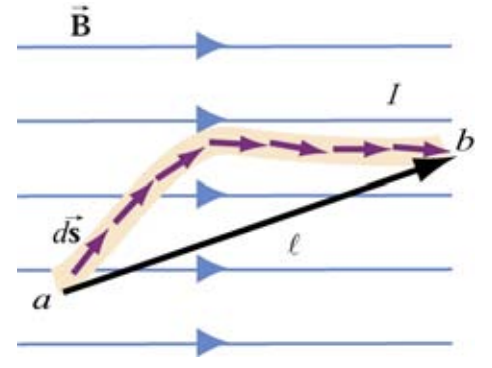
\includegraphics[scale=0.6]{arbitrary}
	\caption{Wire of arbitrary shape in a magnetic field.}
	\label{fig:arbitrary}
\end{figure}

The magnetic force acting on the segment is \[d\bv[B]{F} = Id\bv{s}\times\bv{B}\] and thus the total force is
\begin{equation}\label{eqn:arbitrary}
	\boxed{\bv[B]{F} = I\int_a^b d\bv{s}\times\bv{B}}
\end{equation}
where $a$ and $b$ represent the endpoints of the wire.

For example, with the figure given above, the integral will integrate to the distance (in a straight line) from $a$ to $b$, call it $l$. The magnetic force on the wire would then be given by \[\bv[B]{F} = I\left(\int_a^bd\bv{s}\right)\times\bv{B} = I\bv{l}\times\bv{B}\] Another interesting case arise when the segment above forms a closed loop, in which case \[\bv[B]{F} = I\left(\oint d\bv{s}\right)\times\bv{B} = \bv{0}\] Which tells us that the net magnetic force on a closed loop is $\bv[B]{F} = \bv{0}$. This, however, does not imply that the magnetic field is conservative. See proof \hyperref[subsec:non-conservative]{here}.

\section{Torque on a Current Loop.}
\section{Magnetic Force on a Dipole.}
\section{The Lorentz Force.}

\section{Appendix.}
\subsection{Magnetic Fields are Non-conservative}
\label{subsec:non-conservative}
From Wikipedia: A \textit{force field} $\bv{F}$, defined everywhere in space (or within a simply-connected volume of space), is called a \textbf{conservative force} or \textbf{conservative vector field} if it meets any of these three equivalent conditions (for proof of equivalence, see \href{https://en.wikipedia.org/wiki/Conservative_force#Mathematical_description}{here}):
\begin{enumerate}
	\item The curl of $F$ is the zero vector: $\nabla\times\bv{F} = \bv{0}$
	\item There is zero net work done by the force when moving a particle through a trajectory that starts and ends in the same place: $W \equiv \oint_C \bv{F}\cdot\, d\bv{r} = 0$
	\item The force can be written as the negative gradient of a potential, $\Phi$: $\bv{F} = -\nabla\Phi$
\end{enumerate}
The term conservative force comes from the fact that when a conservative force exists, it conserves mechanical energy. The most familiar conservative forces are gravity, the electric force (in a time-independent magnetic field, see Faraday's law), and spring force.

Many forces (particularly those that depend on velocity) are not force fields. In these cases, the three statements above are not equivalent. We have seen that magnetic force satisfies condition $2$, but does not satisfy condition $3$, and condition $1$ is not even defined. The magnetic field is not a force field because vector fields are functions that take one single vector value at each position, and the magnetic force $\bv{F} = q\bv{v}\times\bv{B}(\bv{r})$ also depends on the velocity of the particle that is experiencing the force (which serves as a second parameter). However, you could ask, instead, for the magnetic force on a particle with a given velocity, which itself may or may not depend on the position, i.e. $\bv{v} = \bv{v}(\bv{r})$ (where that dependence may just be a constant), in which case you'll get a map \[\bv{F}\colon\bv{r}\mapsto\bv{F}(\bv{r}) = q\bv{v}(\bv{r})\times\bv{B}(\bv{r})\] that does have a unique value at each position and which therefore does define a vector field, of which you can ask e.g. whether it's conservative or not. However, until you actually define what velocity dependence $\bv{v}(\bv{r})$ you want to take, none of those terms are applicable.

\section{Exercises.}
\subsection{Warm-up}
\subsection{Conceptual Questions}
\subsection{More Practice}



\end{document}
